\subsection{EDA}

Exploroatory Data Analysis (EDA) provides an overview of what could be done to the data to improve the models' performance. 

\subsubsection{Data Profiling and Malformed Entries}

All of the columns and their data types can be seen at table \ref{tab:columns}. When checking for null values, all other columns are free from null values other than \texttt{Income}. Upon inspection, there seems to be no connection with all the other attributes of the entries with null valued `Income`. As far as inspection and analysis goes, they seem to just be malformed entries. 

\texttt{Marital\_Status} also has multiple entries that could be thought of as different, similar, or sometimes even a malformed entry. In the list of unique values for the column, the values are \texttt{Divorced, Single, Married, Together, Widow, YOLO, Alone, Absurd}. Upon listing the value counts, \texttt{Alone, YOLO, Absurd} have very few entries which could be considered as outliers. There have been thoughts of merging some of these entries to the other entries with bigger value counts; e.g. \texttt{Single} would adopt the records with \texttt{Alone}, etc. However, the problem lies wherein there is no way to deduce their backgrounds and whether or not the adopting categories should take in the outliers. To further explain, there is no way to tell if a record that is \texttt{Alone} might have came from a divorced background or if they simply are single. However, a further explanation of the choice between data integrity and model performance will be provided later in experimentations.

\subsubsection{Univariate Analysis}

The skewness and imbalance of data attributes become apparent upon further isolated inspection. Firstly, \texttt{Income}'s central tendencies at table \ref{tab:income desc}

To put into perspective figure \ref{fig:income hist} shows the distance of the max value from the mean of the distribution with a skewness of 6.763487372811116

The decision to remove outliers depends on the models' robustness to outliers, which will be further explained in the experimentation section.

\begin{table}[H]
    \caption{Income column's descriptive statistics}
    \label{tab:income desc}
    \centering
    \begin{tabularx}{0.7\linewidth}{l>{\raggedleft\arraybackslash}X}
        \toprule
        Statistic & Value\\
        \midrule
        count & 2216 \\
        mean & 52247.251354\\
        std & 25173.076661\\
        min & 1730\\
        25\% & 35303\\
        50\% & 51381.5\\
        75\% & 68522\\
        max & 666666\\
        \bottomrule
    \end{tabularx}
\end{table}

\begin{figure}[H]
    \centering
    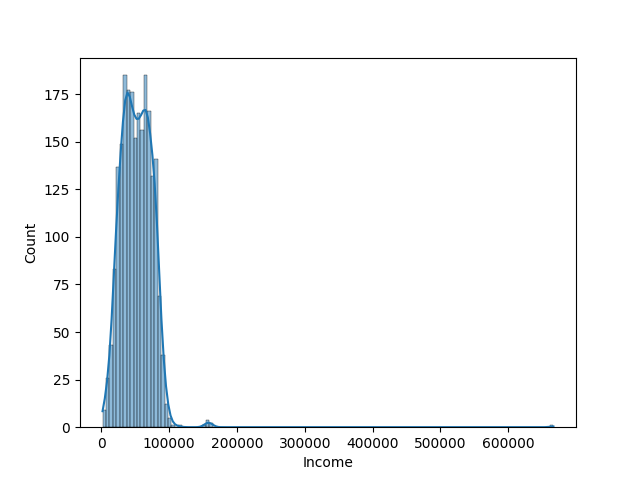
\includegraphics[width=\linewidth]{figures/income_histplot.png}
    \caption{histogram of Income values}
    \label{fig:income hist}
\end{figure}

For \texttt{Education}, although \texttt{Basic} records could be considered as outliers, removing them may misrepresent the dataset.

% \begin{figure}[H]
%     \centering
%     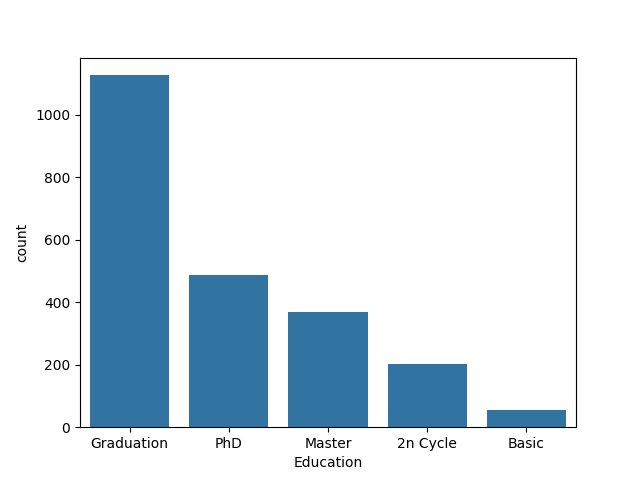
\includegraphics[width=\linewidth]{figures/education_barplot.png}
%     \caption{Bar plot of value counts of the Education column}
%     \label{fig:educ bar}
% \end{figure}

\subsubsection{Bivariate Analysis}

The relationships of attributes to each other are also worth considering to look at. Given that the analysis of these attributes will later be interpreted by the models, this will be discussed in the later sections.

Looking at the scatterplot for the income per year of birth, ignoring the outliers, it seems that there seems to be an equal distribution for each year. Looking around the years 1970 to 1980, there seems to be a few entries where the recorded income is higher than the usual. 

\begin{figure}[H]
    \centering
    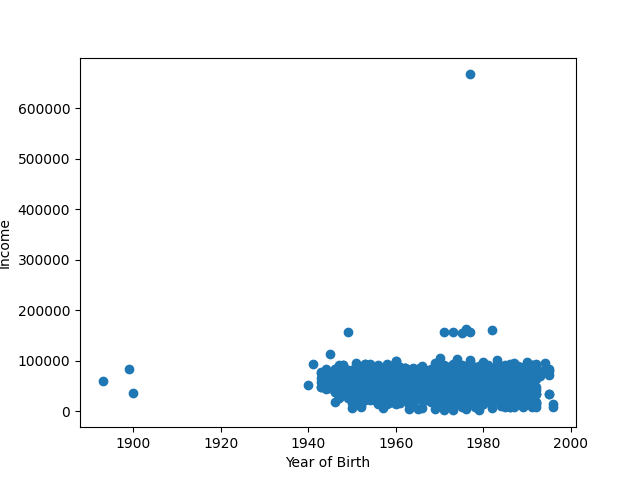
\includegraphics[width=\linewidth]{figures/income_per_yob.png}
    \caption{Scatterplot of income per year of birth}
\end{figure}

Regarding education, when categorized and calculated for central tendencies, \texttt{Basic} provides the lowest average income, while a \texttt{PhD} provides the highest average. However, according to table \ref{tab:educ mean std}, Basic education seems to be the most stable when it comes to delivering a salary based on the standard deviation. PhD education, although high in the average salary, is also very high in standard deviation. This could be seen at the $min$ and $max$ of each category where the minimum income of someone with PhD degree can be as low as 4023 while someone with basic education can be sure to have a salary that is atleast 7500.

\begin{table}[H]
    \caption{Descriptive statistics for each unique value in the Education column}
    \label{tab:educ mean std}
    \begin{tabularx}{\linewidth}{l|>{\centering}X>{\centering}X>{\centering}X>{\centering\arraybackslash}X}
        \toprule
        Education & $\bar x$ & $\sigma$ & min & max \\
        \midrule
        2n Cycle & 47633.19 & 22119.08 & 7500 & 96547\\
        Basic & 20306.26 & 6235.07 & 7500 & 34445\\
        Graduation & 52720.37 & 28177.19 & 1730 & 666666\\
        Master & 52917.53 & 20157.79 & 6560 & 157733\\
        PhD & 56145.31 & 20612.98 & 4023 & 162397\\
        \bottomrule
    \end{tabularx}
\end{table}

\begin{figure}[H]
    \centering
    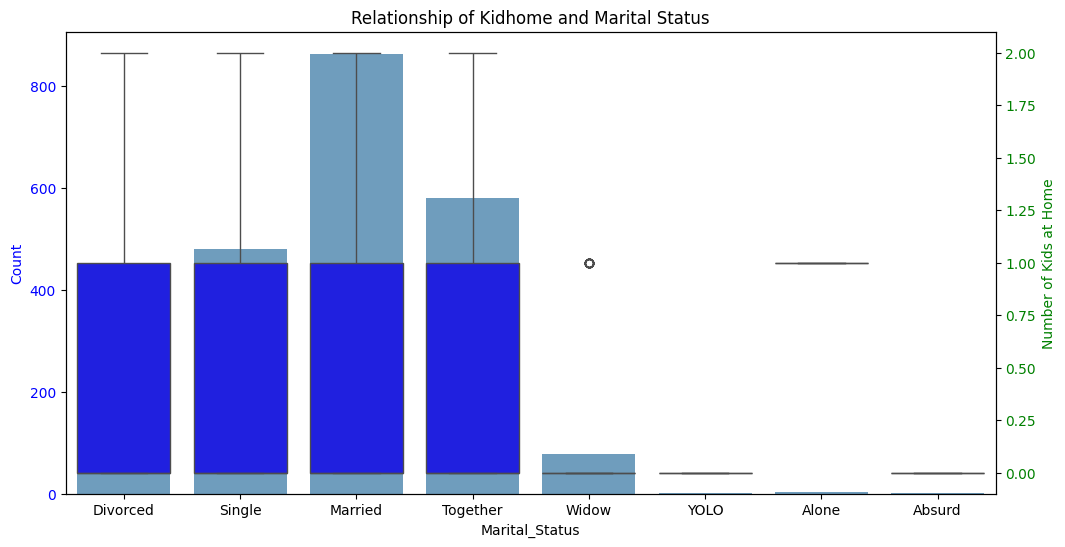
\includegraphics[width=\linewidth]{figures/kidhome_maritalstatus.png}
    \caption{Relationship of Kidhome and Marital Status}
    % \label{fig:income hist}
\end{figure}

The graph illustrates that \texttt{Divorced}, \texttt{Single}, \texttt{Married}, and \texttt{Together} statuses have higher counts compared to \texttt{Widow}, \texttt{YOLO}, \texttt{Alone}, and \texttt{Absurd}, which have fewer individuals. This visualization can help to give meaninful insights on the count and average of the number of children present in the customers' household. For instance, \texttt{Alone} has the highest average among the marital statuses but has a very low count. Displaying their average only can be misleading, which must be avoided as much as possible.

\begin{figure}[H]
    \centering
    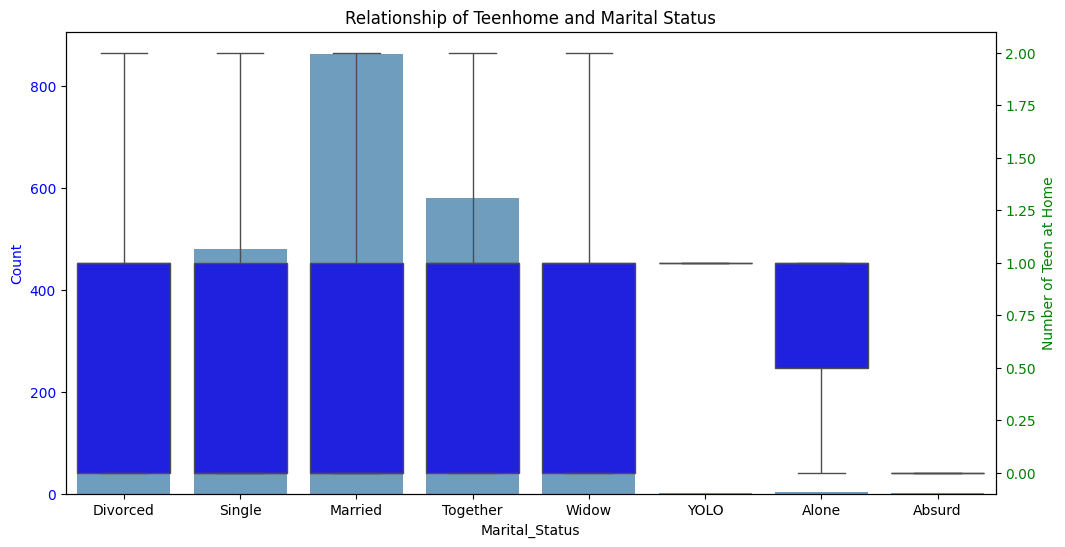
\includegraphics[width=\linewidth]{figures/teenhome_maritalstatus.png}
    \caption{Relationship of Teenhome and Marital Status}
    % \label{fig:income hist}
\end{figure}

Similar with the graph of the relationship of kids at home and marital status, the graph of \texttt{Teenhome} and \texttt{Marital\_Status} resulted with a greater number of individuals with marital statuses of \texttt{Divorced}, \texttt{Single}, \texttt{Married}, and \texttt{Together}. In contrast, \texttt{Widow}, \texttt{YOLO}, and \texttt{Absurd} categories have significantly fewer individuals. Also, the \texttt{Married} category appears to have the highest average number of teenagers at home. This chart help in understanding the influence of marital status on the number of teenagers, which can provide valuable insights during feature engineering in the preprocessing phase.

\subsubsection{Correlation Analysis}

Using correlation analysis during the exploratory data analysis phase can be help identify relationships between variables and inspire the creation of new features. Understanding the impact of each feature to each other can help in building more efficient predicitve models.

    3.1.5.1 Correlation between Income and Education. An investigation was conducted to analyze the relationship between \texttt{Income} and various \texttt{Education} levels. The \texttt{Education} was converted into distinct binary variables through one-hot encoding, so it can be used to quantify the correlation between each educational levels and \texttt{Income}. Individuals with a \texttt{Basic} education level exhibit a negative correlation (-0.200576), suggesting that this group tends to have a lower income levels compared to the baseline category. Meanwhile, the \texttt{PhD} category showed a positve correlation (0.081552), indicating that these individuals tend to earn more than the baseline, implying that the higher educational attainment can correlate with higher income levels. Lastly, the \texttt{2n Cycle}, \texttt{Graduation}, and \texttt{Master} education levels showed correlations of -0.057745, 0.018935, and 0.011827, respectively, with \texttt{Income}. These figures suggest that they only have a slightly correlation with \texttt{Income} values.

    These results exhibit a weak correlation between these two variables. This observation suggests that education alone is not a strong predictor of income levels within the dataset. This can become a basis to decide in which approach is the most appropriate during the preprocessing phase.

    3.1.5.2 Correlation between Income and Marital Status. Similar to the examination of education's influence on income, correlation analysis between \texttt{Marital\_Status} and \texttt{Income} was explored to provide meaningful insights that can be later used in the experiments. The \texttt{Marital\_Status} was also converted into distinct categories through one-hot encoding for analysis with \texttt{Income} which yielded informative insights. Marital statuses \texttt{Absurd} (0.024026), \texttt{Divorced} (0.007975), and \texttt{Together} (0.0234425) both show slight positive correlations with \texttt{Income}, which suggests that individuals with these marital statuses tend to have marginally higher incomes compared to the baseline category. While, marital status \texttt{Widow} (0.031706) exhibit positive correlation as well, but has weak relationship. This status presents the highest positive correlation among the statuses. Lastly, marital statuses \texttt{Alone} (-0.012374), \texttt{Married} (-0.016479), \texttt{Single} (-0.025843), and \texttt{YOLO} (-0.004556) are negatively correlated with 'Income'. These finding imply that individuals with these marital statuses tend to have slightly lower incomes compared to the baseline.

    Similar to the finding with \texttt{Education}, the correlations between \texttt{Income} and \texttt{Marital\_Status} are generally weak. This indicates that \texttt{Marital\_Status} is not a strong predictor of income within the dataset.

\subsubsection{Chi-square test of independence}

Using Chi-square test of independence is suitable in comparing categorical data to see if there is a statistically significant relationship between the two categorical variables.

    3.1.6.1 Association between Income and Education. Customer complaints \texttt{Complain} and education levels \texttt{Education} was investigated to see their association with each other using the Chi-square test of independence. It resulted with a p-value of 0.11620258344593623, which is greater than 0.05. This suggests that there is no significant between the two variables, implying that \texttt{Education} is not a good determinant for customer complaints.

    3.1.6.2 Association between Income and Marital Status. Similar with the observation between customer complaints and education levels, the association between \texttt{Complain} and \texttt{Marital\_Status} was determined through Chi-square test. The test resulted in a p-value of 0.9870342644720567, indicating that there is no significant association between the two variables. Just like education level, marital status does not significantly affect whether customers have lodged complaints.

\subsubsection{ANOVA Test}

ANOVA tests were conducted to evaluate the relationship between \texttt{Marital\_Status} and the variables \texttt{Kidhome} and \texttt{Teenhome}. These tests are important to understand how the number of kids and teenagers at home may vary across different marital statuses, which could potentially influence the development of the models and inspire to create new features.

    3.1.7.1 Analysis between Kidhome and Marital Status. The ANOVA test for \texttt{Kidhome} by \texttt{Marital\_Status} resulted to a F-statistic of 2.8150772422212915 and a p-value of 0.006399583359671683. A high F-value suggests that there are significant differences between the groups, while the p-value is below the significance level of 0.05. This suggests that there is a significant differences in the average number of children at home among different marital status. This means that the \texttt{Marital\_Status} has a huge effect on the \texttt{Kidhome} variable.

    3.1.7.2 Analysis between Teenhome and Marital Status. The ANOVA test for \texttt{Teenhome} by \texttt{Marital\_Status} resulted to a F-statistic of 4.461449687945867 and a p-value of approximately 0.000060909780334068225. This p-value indicates that the number of teenagers in the household significantly varies by marital status. Given this significant p-value, it is safe to say that \texttt{Marital\_Status} plays a bigger role in determining the \texttt{Teenhome} variable compared to \texttt{Kidhome}. 

\subsubsection{Analysis for \texttt{Mnt[.]+} and \texttt{Num[.]+} Columns}

\begin{figure}[H]
    \centering
    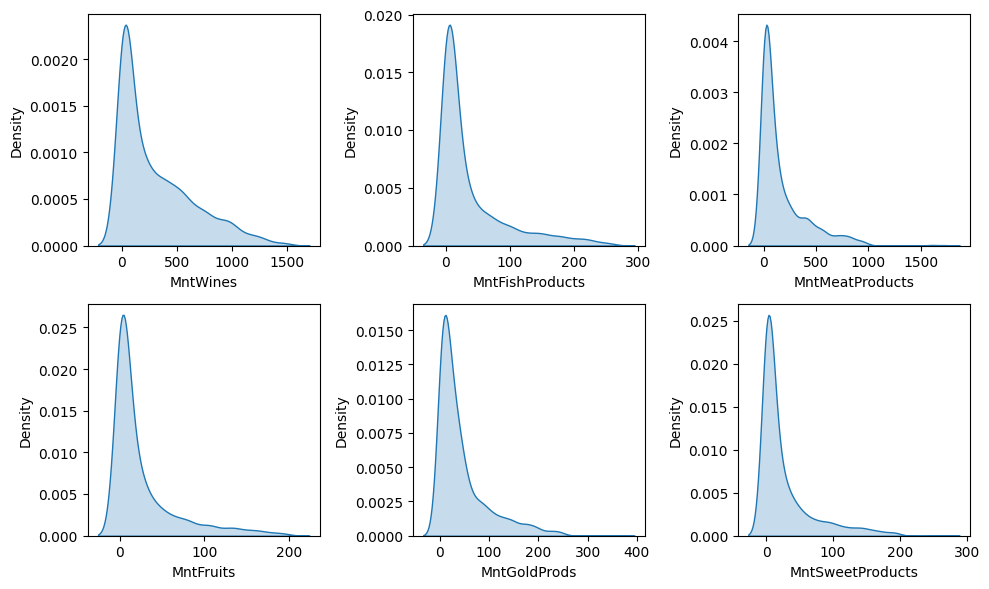
\includegraphics[width=\linewidth]{figures/spending_products.png}
    \caption{Distribution of Customer Spending Across Various Product Categories}
    % \label{fig:income hist}
\end{figure}

The illustration consists of six kernel density estimation (KDE) plots, each representing the distribution of spednging across different products, such as wines, fish products, meat products, fruits, gold products, and sweet products. Using KDE plots for these variables are helpful to visualize their distribution shape to identify the skewness of each spending category. All distributions are right-skewed, indicating that the majority of customers spend less in these categories. There is also a noticeable spending habits based on this graphs. For instance, \texttt{MntWines} show a potential for higher customer spending than other categories.

\begin{figure}[H]
    \centering
    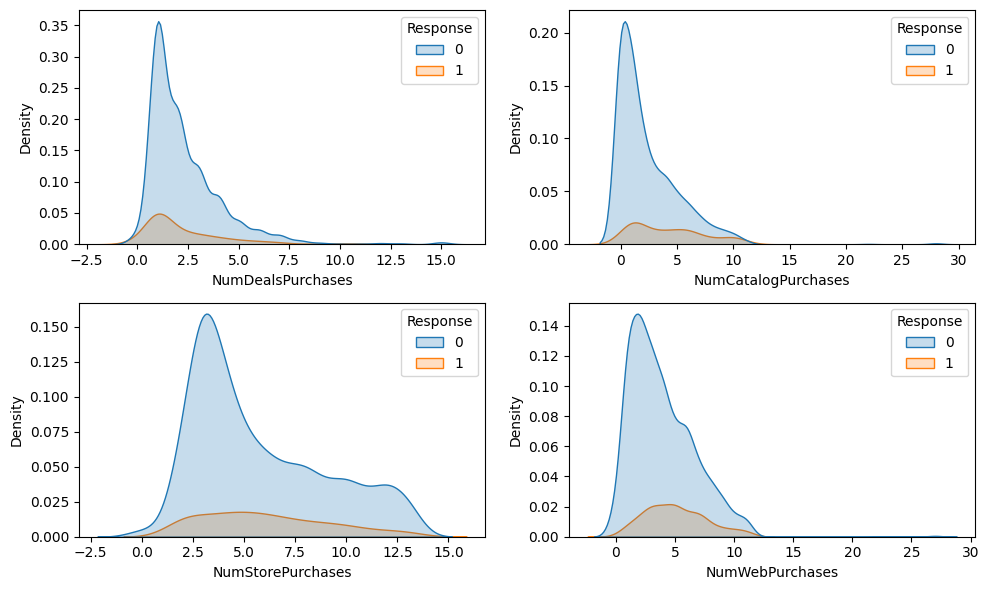
\includegraphics[width=\linewidth]{figures/num_purchases.png}
    \caption{Differences in Customer's Purchasing Behavior Across Different Channels'}
    % \label{fig:income hist}
\end{figure}

Similar with the illustration for the distribution of customer spending, KDE plots were used to illustrate the distribution of different types of purchases made by customers. Additionally, the customers' response to the campaign were segmented to see the pattern of their purchasing behaviors who responded to the campagaign and who did not. In general, those who availed the promo exhibit flatter distibutions in their purchasing behaviors across different channels which means that they are more likely to explore and buy using different channels. While the customers who did not avail the promo tend to buy less and not venture into different types of purchases than those who did.

\begin{figure}[H]
    \centering
    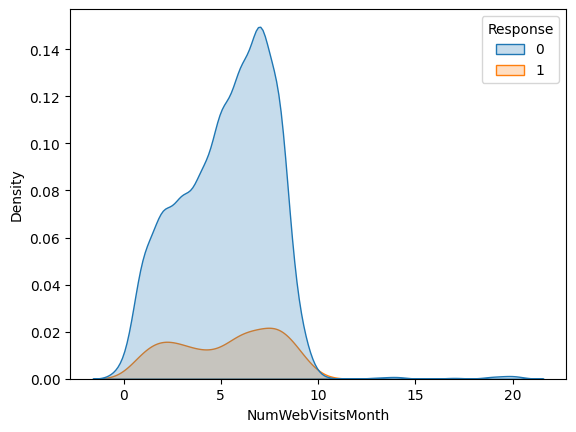
\includegraphics[width=\linewidth]{figures/numwebvisits.png}
    \caption{Density Plot of Monthly Website Visits by Respone'}
    % \label{fig:income hist}
\end{figure}

The graph suggests that customers who did not avail the promo actually visit the website more frequently than those who got the promo. This could mean that those who did not avail are looking for deals in the website but failed to find what they want or those who got the promo are already satisfied customers that don't need to visit the website as often. This can be helpful in understanding the behavior of the customers and create meaningful strategies to create an accurate predictive model.
